\input{../header}

\begin{document}
%


%\onehalfspacing
\allowdisplaybreaks
%##################################################################
\section{PS\#7: Work and pressure - \red{Answer key} }

\everymath{\displaystyle}
\begin{enumerate}[leftmargin=0pt]

\item (\href{https://activecalculus.org/single/sec-6-4-physics.html#BsF}{Example 6.4.6}) Consider a trapezoid-shaped dam that is 60 feet wide at its base and 90 feet wide at its top, and assume the dam is 25 feet tall with water that rises to within 5 feet of the top of its face. Water weighs 62.4 pounds per cubic foot. How much force does the water exert against the dam? (Set up by measuring $h$ from the bottom of the dam up.)

\begin{center}
    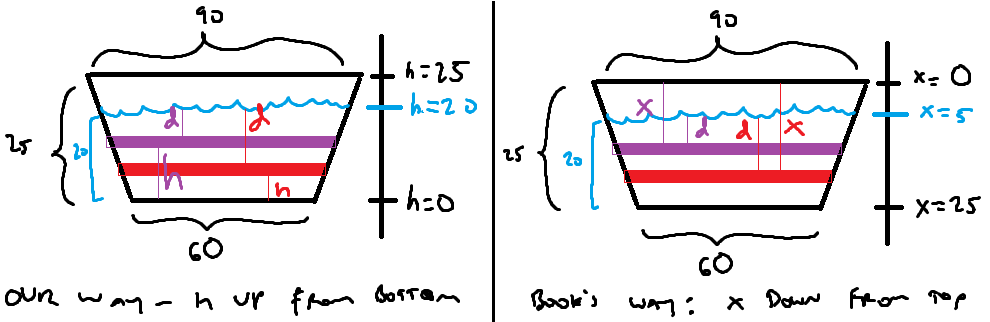
\includegraphics[width=\textwidth]{../images/example-6-4-6.png}
\end{center}
\begin{enumerate}
    \item[E.] Write an equation for $w(h)$, the width of the slice at height $h$.

    \begin{red}
    We know these points:
        $
\begin{array}{l||ll}
h & 0  & 25 \\\hline
w & 60 & 90
\end{array}
        $ \quad
        Therefore $w(h) = 60 + \tfrac65 h$.
    \end{red}
    \item[F.] Write an equation for $\Delta A(h)$, the area of the slice at height $h$. \begin{red}
        $\Delta A(h) = w(h)\cdot \Delta h = (60 + \tfrac65 h)\Delta h$.
    \end{red}
    \item[G.] Write an equation for $P(h)$, the pressure at height $h$. Remember that $P(d) = 62.4d$. How are $d$ and $h$ related?

    \begin{red}
        Looking at the picture, $d + h = 20$, so $d = 20 - h$. Therefore, $P(h) = 62.4\cdot(20-h).$
    \end{red}
    \item[H.] Write an equation for $\Delta F(h)$, the force that the slice at height $h$ feels. 
    
    \begin{red}
        $\Delta F(h) = P(h)\cdot\Delta A(h) = 
        \left[ 62.4\cdot(20-h) \right]\cdot\left[(60 + \tfrac65 h)\Delta h\right]$.
    \end{red}
    \item[I.] Finally, write down a definite integral that computes the total force on the dam. Label your bounds of integration.

    \begin{red}
    The bounds of integration are from the bottom of the dam, $h=0$, to the top of the water, $h=20$.
        \[F_\text{total} = \int_{h=0}^{h=20}62.4\cdot(20-h) \cdot \left(60 + \dfrac65 h\right)\ dh.\]
    \end{red}
\end{enumerate}
\vspace{-2em}
\item (Example 6.4.6, book's setup)
\begin{enumerate}
    \item[E.] The book says that it is ``straightforward'' to see that $w(x) = 2\left(45 - \tfrac35 x\right)$. How did they come up with this equation for $w(x)$?
    
    \begin{red}
        The book has put the positive $x$-axis pointing down through the center of the dam, so they're looking at $y$ as half the width. We know these points:
        $
\begin{array}{l||ll}
x & 0  & 25 \\\hline
y & 45 & 30
\end{array}
        $\quad
        Therefore $y(x) = 40 + \tfrac35 x$, so that $w(x) = 2\left(45 - \tfrac35 x\right)$. 
    \end{red}
    \item[F.] What is the book's equation for $\Delta A(x)$, and how did they come up with it? (The book chooses to call this $A\slice$).
    \begin{red}
        $\Delta A(x) = w(x)\cdot\Delta x =  2\left(45 - \tfrac35 x\right)\Delta x$. 
    \end{red}
    \item[G.] What is the book's equation for $P(x)$ (aka $P\slice$), the pressure at location $x$? How did they come up with it?

    \begin{red}
        Again, $P(d) = 62.4d$, so we need to know the relationship between $x$ and $d$. Since the water level is 5 feet down from the top of the dam, $d+5=x$, so $d = x-5$. Therefore $P(x) = 62.4\cdot(x-5)$.
    \end{red}
    \item[H.] What is the book's equation for $\Delta F(x)$ (aka $F\slice$), the force that the slice at location $x$ feels?
    
    \begin{red}
        $\Delta F(x) = P(x)\cdot \Delta A(x) = [62.4\cdot (x-5)]\cdot\left[2\left(45 - \tfrac35 x\right)\Delta x\right]. $
    \end{red}
    \item[I.] What is the book's definite integral for the total force on the dam? Why are their bounds of integration correct?

    \begin{red}
        The bounds of integration are from the top of the water, $x=5$, to the bottom of the dam, $x=25$.
        \[F_\text{total} = \displaystyle\int_{x=5}^{x=25} 62.4\cdot(x-5)\cdot\left(2\left(45 - \dfrac35 x\right)\right)\ dx. \]
    \end{red}
\end{enumerate}

\item (\href{https://activecalculus.org/single/sec-6-4-physics.html#wrN}{AC 6.4 Exercise 7}) A cylindrical tank, buried on its side, has radius 3 feet and length 10 feet. It is filled completely with water whose weight density is 62.4 lbs/ft$^3$, and the top of the tank is two feet underground.

\begin{red}
    Note: I'm providing both ``delta-style'' and ``slice-style'' versions of each setup, so you can see the setup both ways, depending on what you prefer.
\end{red}

\begin{enumerate}
    \item Set up, but do not evaluate, an integral expression that represents the amount of work required to empty the top half of the water in the tank to a truck whose tank lies 4.5 feet above ground.
    
    \begin{red}
    First step: draw a picture and draw a slice. Your picture may of course be a little different -- perhaps in particular you may have chosen to draw a length down from the top of the tank to the slice, rather than the length I've drawn from the center up to the slice. I have both a picture of the overall tank situation and a picture of the end of the tank to help me figure out the relationship between the width of the slice and its height up from the center.
    
    \begin{center}
        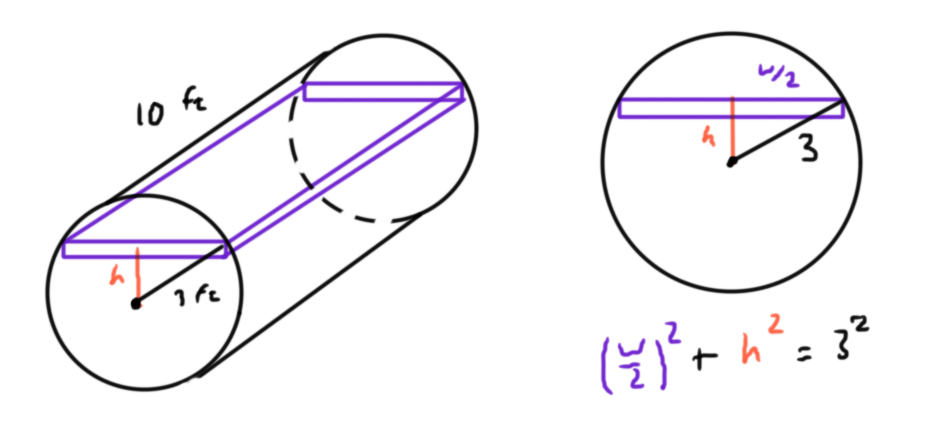
\includegraphics[width=0.7\textwidth]{../images/fig-6.4.7.a.png}
    \end{center}
    Now we can figure out the work done to lift a slice. Notice that I'm using capital $W$ for ``work'' and lowercase $w$ for ``width'' -- this is moderately annoying but I believe in you. The work done to lift a slice is the force needed to lift the slice times the distance that slice will be lifted:
    \begin{align*}
        W\slice &= F\slice \cdot D\slice
        & \Delta W = \Delta F \cdot D(h)\\
        &= (V\slice\cdot\rho)\cdot D\slice 
        &= (\Delta V \cdot \rho)\cdot D(h) \\ 
        &= (\ell\cdot w\slice \cdot \Delta h\cdot 62.4)\cdot D\slice 
        &= (\ell\cdot w(h)\cdot\Delta h\cdot 62.4)\cdot D(h)\\
        \intertext{The width of the slice depends on $h$ in the way illustrated in the diagram. I've solved the equation I wrote for $w$:}
        &= (10\cdot 2\sqrt{9-h^2}\cdot \Delta h \cdot 62.4)\cdot D\slice
        &= (10\cdot 2\sqrt{9-h^2}\cdot \Delta h \cdot 62.4)\cdot D(h)\\
        \intertext{The slice at height $h$ needs to be lifted by $3-h$ to get to the top of the tank, then by 2 to get to ground level, then by 4.5 to get into the truck.}
        &= (10\cdot 2\sqrt{9-h^2}\cdot \Delta h \cdot 62.4)\cdot (3-h+2+4.5) \\
        &= (10\cdot 2\sqrt{9-h^2}\cdot \Delta h \cdot 62.4)\cdot (9.5-h) \\
        \text{Unit check:\quad \quad} 
        &= (\underbrace{10\cdot}_{\text{ft}}
        \underbrace{2\sqrt{9-h^2}}_{\text{ft}}\cdot 
        \underbrace{\Delta h}_{\text{ft}} \cdot 
        \underbrace{62.4}_{\text{lb / ft}^3})\cdot 
        \underbrace{(9.5-h)}_{\text{ft}} \quad & \text{Yay, that's the right units.}
    \end{align*}
    Now we need to integrate from the center of the tank to the top of the tank. That's from $h=0$ to $h=3$. Therefore, the integral computing the amount of work is
    \[W_\text{total} = \int_{h=0}^3 (10\cdot 2\sqrt{9-h^2} \cdot 62.4)\cdot (9.5-h)\ dh.  \]
    \end{red}
    
    \item With the tank now only half-full, set up, but do not evaluate an integral expression that represents the total force due to hydrostatic pressure against one end of the tank.
    
    \begin{red}
    First step: draw a picture and draw a slice. Your picture may of course be a little different -- perhaps in particular you may have chosen to draw a length up from the bottom of the tank to the slice, rather than the length I've drawn from the center down to the slice. 
    
    \begin{center}
        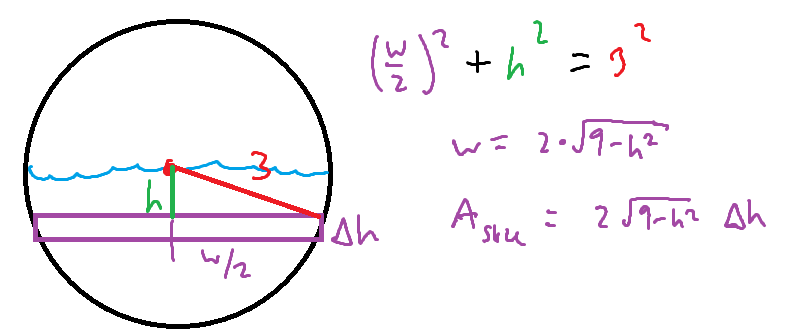
\includegraphics[width=0.7\textwidth]{../images/fig-6.4.7.b.png}
    \end{center}
    Now we can figure out the force due to pressure on that slice, which is the area of that slice multiplied by the pressure on that slice. To compute the pressure, we'll multiply the depth of the slice (which is $h$ according to my diagram, since I'm measuring down from the middle) by the weight of water.
    \begin{align*}
        F\slice &= P\slice \cdot A\slice 
        & \Delta F = P(h) \cdot \Delta A\\
        &= 62.4\cdot h\cdot A\slice
        &= 62.4\cdot h \cdot \Delta A \\ 
        &= 62.4\cdot h \cdot (w\slice\cdot\Delta h) 
        &= 62.4\cdot h \cdot (w(h)\cdot\Delta h) \\
        \intertext{The width of the slice depends on $h$ in the way illustrated in the diagram. I've solved the equation I wrote for $w$:}
        &= 62.4\cdot h \cdot \left(2\sqrt{9-h^2}\cdot \Delta h\right)\\
        \text{Unit check:\quad \quad} 
        &= 
        \underbrace{62.4}_{\text{lb / ft}^3}\cdot
        \underbrace{h}_{\text{ft}}\cdot
        \underbrace{2\sqrt{9-h^2}}_{\text{ft}}\cdot
        \underbrace{\Delta h}_{\text{ft}}
         \quad & \text{Yay, that's the right units.}
    \end{align*}
    Now we need to integrate from the center of the tank to the bottom of the tank. According to my diagram, that's from $h=0$ to $h=3$. Therefore, the integral computing the amount of work is
    \[F_\text{total} = \int_{h=0}^3 62.4\cdot h \cdot \left(2\sqrt{9-h^2}\right)\ dh.  \]
    \end{red}
\end{enumerate}

\end{enumerate}
\end{document}